\TUchapter{The proposed method}

This chapter outlines the general proposed method for forensic data extraction from ECMs. It outlines the requirements that such a solution must meet,
and then describes a general method for meeting those requirements. Specifics of the implementation will be laid out in later chapters.

\TUsection{Requirements}

\TUsubsection{Baseline of Trust}

In order to make a full accounting of potential sources of error in any forensic process, it is important to examine the assumptions that the process requires. Standard methods of 
heavy truck evidence extraction assume that the ECM is reporting data faithfully, and that the vehicle network is accurately transmitting the communication to and from the ECM. It also assumes 
the Vehicle Diagnostic Adapter (VDA) is faithfully sending data from the vehicle network to the RP1210 library that is called by the OEM software.

While verifying the correct internal functioning of heavy truck ECMs is beyond the scope of this research, the fidelity of data transmitted across the various networks (CAN bus, serial 
bus and USB) can be easily verified. Both protocols make use of error-correcting codes that detect transmission errors with very high reliability; for example, the CAN 
cyclic redundancy check that is defined in the CAN standard detects all errors from 1 to 5 bits in the data frame, and will detect all but 0.00018\% of 6-bit 
errors in a CAN frame \cite{koopman2004}. This represents a level of certainty that would take many years to experimentally verify because the likelihood of having an undetected error is so low.

\TUsubsection{Protocols}

Because typical ECM data extractions occur over vehicle networks, analysis of their forensic soundness requires consideration of the specifications
of protocols  used for communication over those networks.
In heavy trucks, the networking protocols enumerate and define the various data that are transmitted over the in-vehicle network, which in turn provides clues as to the nature 
of the data present in the ECM. For example, a data type that is rounded to the nearest power of ten (186 rounded to 190, for example) when transmitted on the network might 
indicate that the value stored to and reported by the ECM is rounded in a similar fashion.

\TUsubsection{Authentication}

A cryptographic hash function is an algorithm that generates a “fingerprint” of a given input. This fingerprint is generated in such a way that if a single bit of the input changes, 
roughly half the bits in the output file are altered \cite{schneier1996}. As such, they are commonly used to confirm that data have not been altered. A forensically sound tool should use a hash of 
the extracted truck evidence data to ensure that it has not been altered.

\TUsubsection{Evidence Preservation}

Ideally, a forensic solution would allow the evidence to be preserved indefinitely. While hard disks are fairly inert when not used, heavy truck ECMs are actual computers that 
have some volatile data elements. One example is the ECM's system clock.

Volatile clock data requires a continuous supply of electrical power to avoid being deleted. The on-board 
system clock is important to investigators because it correlates with the timestamps associated with incident records. An exemplar circuit, shown in Figure \ref{fig:clockbatt}, is based around 
the EM Micro V3020 realtime clock, as used in several Detroit Diesel ECMs.  It is important that the actual on-board system clock be preserved, because the system clock is not necessarily synched 
up with standard times and the offset from the standard time must be recorded at the time of investigation.

Though the batteries in ECMs are large, and power drains slowly over time, this is an example of potentially critical information that can be lost if not extracted and preserved.

\begin{figure}[h]
  \centering
  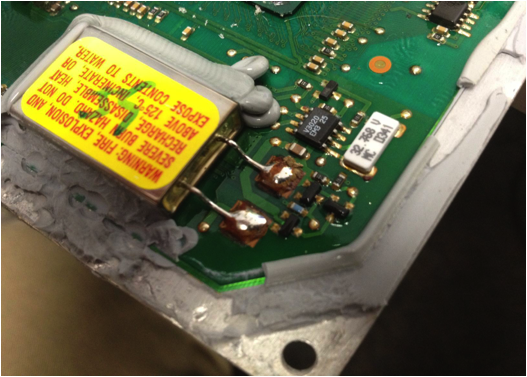
\includegraphics{clockbatt}
  \caption{The real time clock of a Detroit Diesel engine controller with system battery}
  \label{fig:clockbatt}

\end{figure}

\TUsection{The Solution For Secure Extraction}
The solution arrived at was borrowed from the world of computer forensics. In a computer forensic investigation,
a low-level copy of the evidence drive is made; this copy is known as the ``disk image.'' Forensic analysis
is performed on this disk image instead of the original disk, so as to alter the original source evidence as
little as possible.

The goal was to extend this concept to truck ECMs: the information would be extracted exactly one time, and then
replayed for further analysis. The replay traffic information would be stored securely to prevent malicious tampering
or accidental alteration.

\TUsubsection{Software Requirements}

Development of the forensic replay software requires the following steps:

\begin{enumerate}
  \item Record the network traffic produced by the original information extraction process. This may be done either with a vehicle
        network traffic logger, or by logging API calls to the DLC driver.
  \item Decipher any encryption or obfuscation mechanisms obscuring ECM data. Many manufacturers use protocols that encrypt diagnostic
        data, and some are sufficiently well designed that the traffic cannot simply be replayed. Thus, replaying the data requires
        that the encryption can be deciphered.
  \item Store the evidence in a secure manner. If the evidence is stored in such a way that it can be tampered with, the integrity of
        the evidence may be called into question. This is unacceptable in a forensic context.
  \item Respond to information requests identically to the ECM. As the goal is to make a digital ``image'' of the ECM, the forensic system
        must be able to recreate the same traffic that the ECM would.
\end{enumerate}

All of these would ideally be performed in a manner that is as general as possible to minimize development time
supporting additional ECMs.

\TUsubsection{Comparison of method to disk imaging}

The largest difference between the proposed extraction replay method and a forensic disk extraction is obviously
the amount of information extracted. When a disk is imaged, the entire physical contents of the disk (except for
any blocks hidden by a Dynamic Drive Overlay or a Host Protected Area) are extracted. However, a replay of a
software extraction only extracts the information normally accessed during that data  extraction. Accessing more data
would require reading data directly from the ECM's memory chips.

Another difference is that protocols for accessing hard disks are standardized, so one method can be reasonably expected
to work reliably across all commercially available hard disks. ECM data, however, are acessed with proprietary protocols,
that vary from manufacturer to manufacturer, over standard networks. 
Therefore, each individual manufacturer that will be supported requires understanding of the  manufacturer's proprietary protocol extensions.

